\documentclass[11pt,a4paper]{article}

% ---------- Packages ----------
\usepackage[a4paper,top=0.75in,bottom=0.70in,left=0.85in,right=0.85in]{geometry}
\usepackage{newtxtext,newtxmath}
\usepackage{graphicx}
\usepackage{array}
\usepackage{booktabs}
\usepackage{enumitem}
\usepackage{titlesec}
\usepackage{fancyhdr}
\usepackage{setspace}
\usepackage{ragged2e}
\usepackage[hidelinks]{hyperref}
\usepackage{caption}
\usepackage{float}
\usepackage{tabularx}
\usepackage{longtable}
\usepackage[T1]{fontenc}

% ---------- General formatting ----------
\setlength{\parindent}{0pt}
\setlength{\parskip}{4pt}
\setstretch{1.0}
\setlist[itemize]{leftmargin=0.28in,itemsep=1pt,topsep=1pt}
\setlist[enumerate]{leftmargin=0.30in,itemsep=1pt,topsep=1pt}
\AtBeginDocument{\fontsize{10.5}{12.0}\selectfont}

% Chapter headings: match the report's black serif presentation.
\titleformat{\section}
  {\normalfont\fontsize{16}{19}\selectfont}
  {\thesection}{0.6em}{}
\titlespacing*{\section}{0pt}{4pt}{6pt}

\titleformat{\subsection}
  {\normalfont\fontsize{12.5}{15}\selectfont\bfseries}
  {\thesubsection}{0.55em}{}
\titlespacing*{\subsection}{0pt}{5pt}{5pt}

\titleformat{\subsubsection}
  {\normalfont\fontsize{11.5}{14}\selectfont\bfseries}
  {\thesubsubsection}{0.55em}{}
\titlespacing*{\subsubsection}{0pt}{4pt}{4pt}

% "Chapter N" lines are manually inserted to mirror the DOCX.
\newcommand{\chaptertitle}[2]{%
  \vspace*{0pt}%
  {\normalfont\fontsize{22}{25}\selectfont #1\par}%
  \vspace{2pt}%
  \noindent\rule{\textwidth}{0.7pt}\par
  \vspace{7pt}%
  {\normalfont\fontsize{22}{25}\selectfont #2\par}
  \vspace{5pt}%
}

% Figure caption style
\captionsetup[figure]{font=small,labelfont=normal,textfont=it,justification=centering,skip=5pt}

% Header/footer on continuation pages only; chapter pages are kept clean.
\pagestyle{fancy}
\fancyhf{}
\renewcommand{\headrulewidth}{0pt}
\fancyfoot[C]{\small\thepage}

% ---------- Document ----------
\begin{document}

% ============================================================
% COVER
% ============================================================
\thispagestyle{empty}
\vspace*{0.65in}
\begin{center}
{\fontsize{18}{22}\selectfont\bfseries UCS503P -- Software Engineering Project\par}
\vspace{0.22in}
{\fontsize{25}{30}\selectfont\bfseries ResQ: Crisis Coordination Platform for\\
Emergency Response\par}
\vspace{0.14in}
{\fontsize{14}{17}\selectfont A Real-Time Emergency Response and Dispatch Management System\par}

\vspace{0.45in}
{\fontsize{14}{17}\selectfont\bfseries MID-SEMESTER EVALUATION REPORT\par}

\vspace{0.30in}
{\fontsize{12}{15}\selectfont
Submitted by:\par
\vspace{0.08in}
1024170226\quad Gurnoor Singh Marok\par
1024170043\quad Rishi Gupta\par
1027170237\quad Tamanna Chadha\par
1024170255\quad Kaif Ahmad\par
\vspace{0.08in}
Group: 3Q24 BE Third Year, CSE\par
\vspace{0.25in}
Submitted to:\par
Dr. Anushka\par
Mid-Semester Evaluation\par
Computer Science and Engineering Department\par
Thapar Institute of Engineering and Technology, Patiala\par
}
\end{center}

\newpage

% ============================================================
% CONTENTS
% ============================================================
\thispagestyle{empty}
{\fontsize{22}{26}\selectfont Contents\par}
\vspace{8pt}

\begin{tabularx}{\textwidth}{@{}Xr@{}}
\textbf{1\quad Introduction} & 3\\
\quad 1.1\quad Background and Context & 3\\
\quad\quad 1.1.1\quad Problem Statement & 3\\
\quad 1.2\quad Project Objectives & 3\\
[2pt]
\textbf{2\quad Methodology and Design} & 4\\
\quad 2.1\quad System Architecture & 4\\
\quad\quad 2.1.1\quad High-Level Design & 4\\
\quad\quad 2.1.2\quad Technical Stack & 4\\
\quad 2.2\quad UML Diagrams & 4\\
\quad\quad 2.2.1\quad Use Case Diagram & 5\\
\quad\quad 2.2.2\quad Class Diagram & 6\\
\quad\quad 2.2.3\quad Sequence Diagram & 7\\
\quad\quad 2.2.4\quad Activity Diagram & 8\\
\quad 2.3\quad Implementation Details & 9\\
\quad\quad 2.3.1\quad Module 1: Core Functionality & 9\\
\quad\quad 2.3.2\quad Module 2: Secondary Features & 9\\
[2pt]
\textbf{3\quad Results and Evaluation} & 10\\
\quad 3.1\quad Testing Methodology & 10\\
\quad 3.2\quad Performance and Verification Metrics & 10\\
\quad 3.3\quad Analysis & 10\\
[2pt]
\textbf{4\quad Conclusion} & 11\\
\quad 4.1\quad Summary of Work & 11\\
\quad 4.2\quad Key Findings & 11\\
\quad 4.3\quad Future Work and Recommendations & 11\\
\quad 4.4\quad Final Remarks & 11\\
[2pt]
\textbf{Bibliography} & 12
\end{tabularx}

\newpage

% ============================================================
% CHAPTER 1
% ============================================================
\chaptertitle{Chapter 1}{Introduction}

\subsection{1.1\quad Background and Context}

Emergency and disaster response is fundamentally a coordination problem before it is a technology problem. During a local emergency, the difficulty is rarely in collecting a report: a form and a map pin solve that initial part of the problem. The more difficult task is coordinating independent actors who hold partial information and may have different priorities, including affected people, volunteers, non-governmental organizations (NGOs), resource providers, and administrators.

Response capacity during a crisis is scarce. A request that receives duplicate attention while another remains unseen represents capacity that has not been used effectively. ResQ addresses this gap through a shared operational view of requests, responders, locations, and status.

\subsubsection{1.1.1\quad Problem Statement}

Existing ad hoc approaches to local emergency coordination, such as phone calls, spreadsheets, messaging groups, and disconnected organizational dashboards, exhibit several recurring failure modes:

\begin{itemize}
\item \textbf{Duplicated or wasted effort:} Two responders may act on the same request while another request remains unanswered because the actors cannot reliably observe one another's claims.
\item \textbf{Fragmented visibility:} Different roles may work from separate views, making it difficult to maintain a synchronized understanding of request status.
\item \textbf{Unmatched partial resources:} Some emergency needs require combining contributions from multiple providers; simple request/response record-keeping does not model this well.
\item \textbf{Absence of an accountability loop:} A responder should not be the only party deciding that assistance has actually been received.
\item \textbf{Location and contact privacy risk:} Publishing exact coordinates or contact information of affected people can expose them unnecessarily.
\end{itemize}

\subsection{1.2\quad Project Objectives}

For the mid-semester evaluation, the project focuses on a demonstrable core that establishes the coordination model and the security/privacy foundations needed for later real-time features.

\begin{enumerate}
\item Implement a server-enforced five-stage request lifecycle: Unverified $\rightarrow$ Verified $\rightarrow$ In Progress $\rightarrow$ Resolved $\rightarrow$ Closed, with role-based authorization at every transition.
\item Build a unified map-and-log dispatch console that can be used by the five project roles from one codebase, with the available actions adapting to the logged-in role.
\item Protect affected-person location and contact privacy through coordinate fuzzing and authorization-aware response redaction.
\item Provide public emergency submission and request tracking without requiring an account for the initial report, while maintaining a free/open-source or free-tier technology stack.
\end{enumerate}

\newpage

% ============================================================
% CHAPTER 2
% ============================================================
\chaptertitle{Chapter 2}{Methodology and Design}

\subsection{2.1\quad System Architecture}

\subsubsection{2.1.1\quad High-Level Design}

ResQ follows a conventional three-tier web architecture. The React client communicates with a stateless Express REST API, while the API is the only application component that communicates with MongoDB. The database is treated as the source of truth for user and request state.

The central business rule is a forward-only request state machine. Supporting concerns include authorization, privacy redaction, and a status-history audit trail. The frontend uses one shared map-and-rail console rather than five visually separate applications; only the actions available to each role change.

Socket.IO-based real-time propagation and the rule-based matching engine are intentionally treated as later-phase capabilities. This keeps the mid-semester prototype focused on the core lifecycle, privacy, submission, tracking, and dispatch-console functionality.

\subsubsection{2.1.2\quad Technical Stack}

\renewcommand{\arraystretch}{1.25}
\begin{tabularx}{\textwidth}{@{}p{1.2in}p{1.8in}X@{}}
\toprule
\textbf{Layer} & \textbf{Technology} & \textbf{Purpose / Constraint}\\
\midrule
Frontend & React 18 + Vite + TypeScript + Tailwind CSS & Responsive SPA and design-system-based UI\\
Backend & Node.js + Express + TypeScript & REST API, authentication, lifecycle and authorization logic\\
Database & MongoDB + Mongoose & Persistent user/request data and status history\\
Authentication & JWT + bcrypt & Role-aware authentication without a paid identity vendor\\
Maps & react-leaflet + OpenStreetMap & Map-based request visualization without a billed map provider\\
Testing / CI & Vitest, Supertest, GitHub Actions & Automated lifecycle, authorization and API verification\\
Future real-time layer & Socket.IO & Planned cross-dashboard state propagation\\
\bottomrule
\end{tabularx}
\renewcommand{\arraystretch}{1}

\subsection{2.2\quad UML Diagrams}

The UML models below describe the current ResQ prototype. The Use Case diagram includes explicit \texttt{<<include>>} and \texttt{<<extend>>} relationships, while the Class, Sequence, and Activity diagrams are aligned with the same roles, request lifecycle, and privacy-aware architecture.

\newpage

% ============================================================
% USE CASE
% ============================================================
\subsubsection{2.2.1\quad Use Case Diagram}
\begin{figure}[H]
\centering
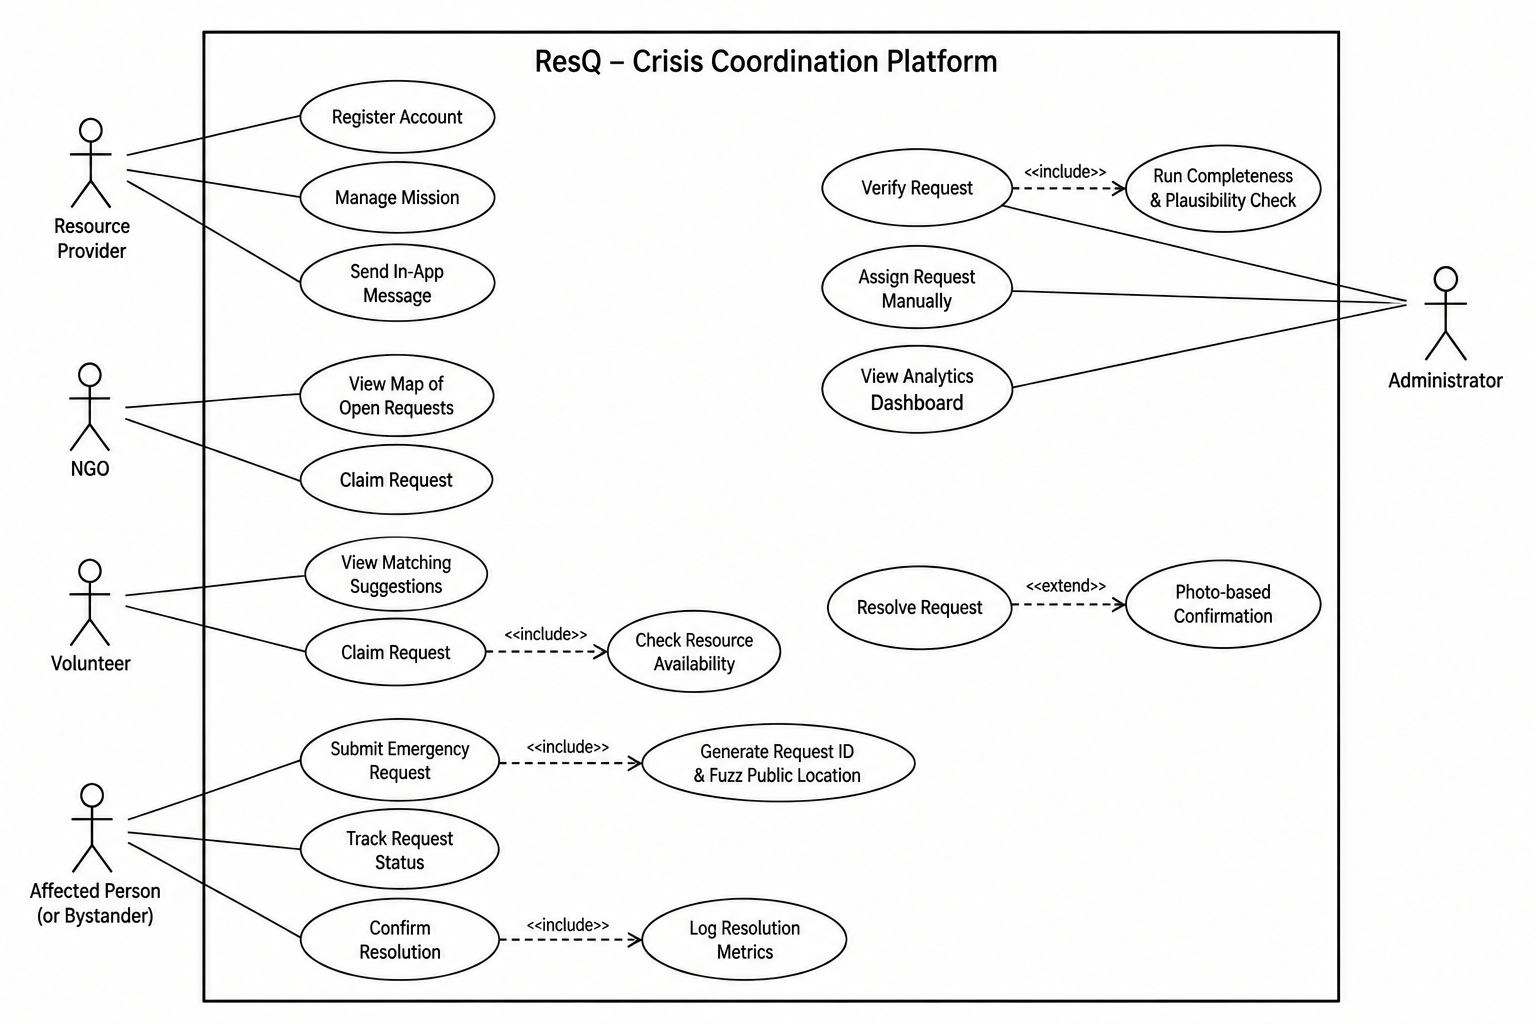
\includegraphics[width=0.96\textwidth,height=8.7in,keepaspectratio]{images/use_case.png}
\caption{ResQ use case diagram}
\end{figure}

\newpage

% ============================================================
% CLASS
% ============================================================
\subsubsection{2.2.2\quad Class Diagram}
\begin{figure}[H]
\centering
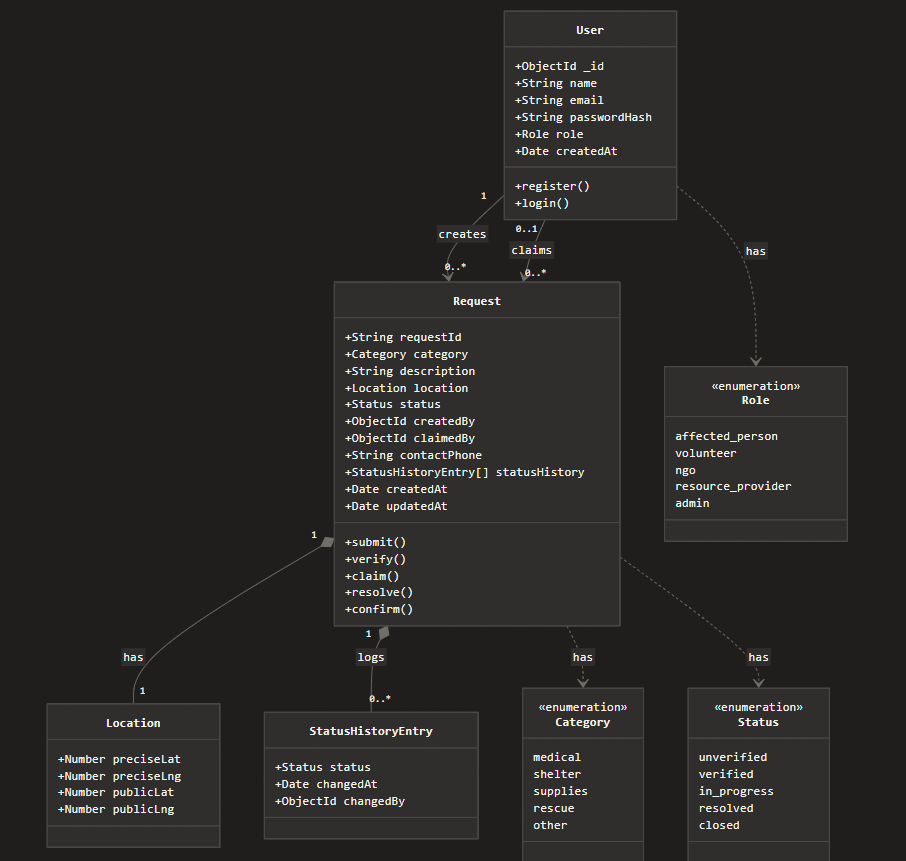
\includegraphics[width=0.88\textwidth,height=9.0in,keepaspectratio]{images/class_diagram.png}
\caption{ResQ class diagram}
\end{figure}

\newpage

% ============================================================
% SEQUENCE
% ============================================================
\subsubsection{2.2.3\quad Sequence Diagram}
\begin{figure}[H]
\centering
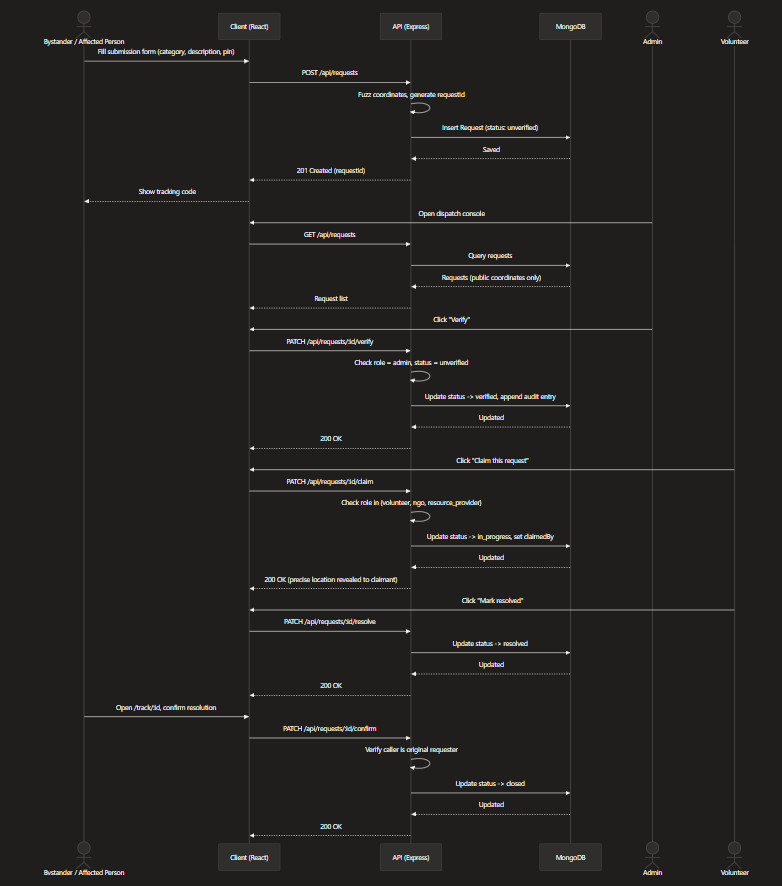
\includegraphics[width=0.88\textwidth,height=9.0in,keepaspectratio]{images/sequence_diagram.png}
\caption{Request submission, retrieval, and responder claim sequence.}
\end{figure}

\newpage

% ============================================================
% ACTIVITY
% ============================================================
\subsubsection{2.2.4\quad Activity Diagram}
\begin{figure}[H]
\centering
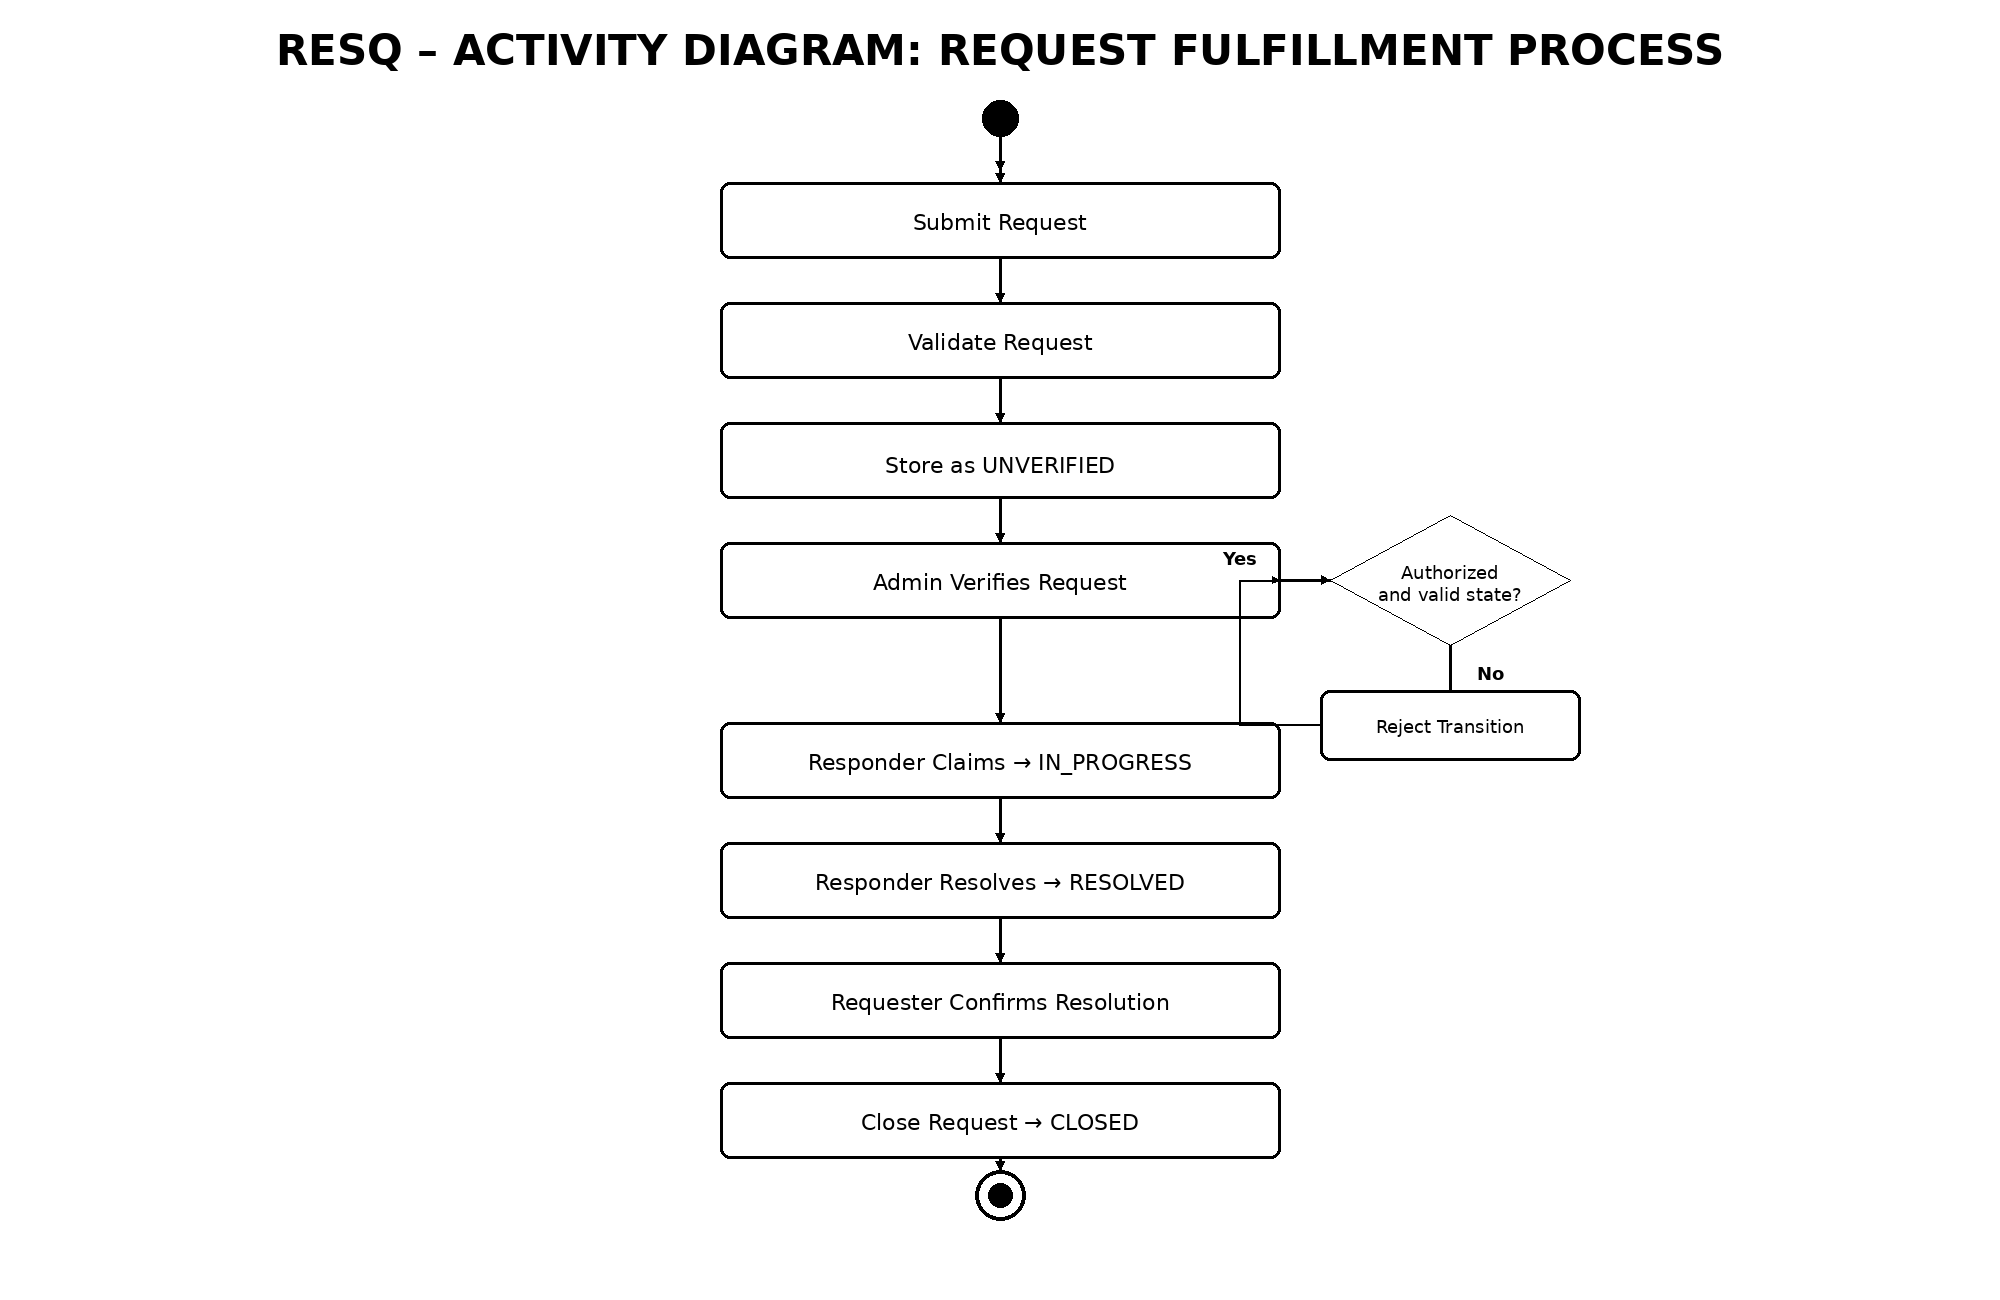
\includegraphics[width=0.92\textwidth,height=7.5in,keepaspectratio]{images/activity_diagram.png}
\caption{Request fulfillment activity flow with authorization/state validation.}
\end{figure}

\newpage

% ============================================================
% IMPLEMENTATION
% ============================================================
\subsection{2.3\quad Implementation Details}

\subsubsection{2.3.1\quad Module 1: Core Functionality}

The User model represents the five project roles: affected person, volunteer, NGO, resource provider, and administrator. Passwords are stored as bcrypt hashes rather than plaintext values. The Request model tracks the request identifier, category, description, status, creator/claimant references, location, and status history.

Location privacy is enforced structurally. Each request contains a precise coordinate pair and a separate fuzzed public coordinate pair. API response sanitization determines whether precise coordinates and contact information may be returned to the caller. Unauthorized callers receive only the public location.

The lifecycle is centralized in transition logic. Each transition checks both the current state and the authorization requirements, preventing skipped or reversed states. Closing a request requires confirmation by the original requester, with the anonymous-request path using the request identifier and phone verification.

\subsubsection{2.3.2\quad Module 2: Secondary Features}

Authentication uses hand-rolled JWT-based sessions and bcrypt password hashing. Public registration is available for project roles except administrator; administrator accounts are provisioned separately.

The frontend provides a shared map-and-rail console. The Leaflet map displays non-closed requests, while the dispatch rail provides filtering and role-specific actions. A mobile-width layout adapts the map/log presentation so that the same workflow remains usable on smaller screens.

The public workflows allow an affected person or bystander to submit a request without logging in and receive a tracking identifier immediately. A tracking page can then display the current lifecycle stage and support the confirmation step. Seed data is used to make the prototype demonstrable without requiring all requests to be entered manually during a presentation.

\newpage

% ============================================================
% CHAPTER 3
% ============================================================
\chaptertitle{Chapter 3}{Results and Evaluation}

\subsection{3.1\quad Testing Methodology}

\begin{itemize}
\item \textbf{Unit and integration testing:} Backend helpers and API behavior are tested using Vitest and Supertest against an in-memory MongoDB instance where applicable.
\item \textbf{Lifecycle verification:} Tests exercise the complete request lifecycle and explicitly cover stage skipping, unauthorized role actions, and attempts to force-close a request.
\item \textbf{Manual walkthrough:} The demonstration flow of submission, verification, claiming, resolution, and confirmation is checked across the project roles.
\item \textbf{Not yet performed:} Formal Playwright end-to-end browser testing, concurrent load testing, and pilot testing with real or simulated end users remain future work.
\end{itemize}

\subsection{3.2\quad Performance and Verification Metrics}

The evaluation below separates properties that are currently verified from metrics that require capabilities or pilot conditions not yet available. This avoids presenting projected values as achieved measurements.

\renewcommand{\arraystretch}{1.35}
\begin{tabularx}{\textwidth}{@{}p{1.35in}p{2.15in}X@{}}
\toprule
\textbf{Metric} & \textbf{Target / Requirement} & \textbf{Status at Mid-Semester}\\
\midrule
Lifecycle transition correctness & All defined transitions enforced; illegal transitions rejected & Achieved -- verified by automated tests\\
Location / contact privacy & No unauthorized exposure of precise coordinates or phone numbers & Achieved -- verified by automated tests\\
Role-based authorization & Actions restricted to intended roles at protected endpoints & Achieved -- verified by automated tests\\
Time-to-Match & Median $\leq$ 15 minutes during pilot & Pending -- requires pilot and matching workflow\\
Cross-dashboard propagation & $<2$ seconds & Not yet applicable -- Socket.IO real-time layer is future work\\
Double-booking rate & 0\% & Not yet measurable -- requires concurrent-user pilot\\
\bottomrule
\end{tabularx}
\renewcommand{\arraystretch}{1}

\subsection{3.3\quad Analysis}

The current checkpoint establishes the core implementation objectives: a server-enforced lifecycle, a unified map-and-log console, and privacy-by-design. The project also maintains the intended free/open-source or free-tier technology constraint.

A key implementation decision is to centralize lifecycle transitions rather than duplicate state checks across individual endpoints. This reduces the chance that a later route bypasses authorization or lifecycle rules. The statusHistory audit trail also provides a foundation for later accountability analysis.

Anonymous submission requires an additional identity-verification path because the requester may not have an account. The request identifier plus phone verification provides the confirmation path without requiring account registration.

\newpage

% ============================================================
% CHAPTER 4
% ============================================================
\chaptertitle{Chapter 4}{Conclusion}

\subsection{4.1\quad Summary of Work}

At this checkpoint, ResQ establishes the core data model, a server-enforced five-stage request lifecycle, role-based authorization, privacy-aware location handling, a unified map-and-log console, public request submission and tracking workflows, and automated backend verification. The implementation remains consistent with the phased development plan and is suitable as a demonstrable mid-semester prototype.

\subsection{4.2\quad Key Findings}

\begin{itemize}
\item Centralizing status-transition logic is essential for enforcing lifecycle order and authorization consistently.
\item A shared console across five roles reduces duplicated UI structure while allowing actions to remain role-specific.
\item Privacy must be implemented at the API/data boundary rather than relying only on frontend hiding.
\item Anonymous submission requires an explicit verification path if the affected person must later confirm resolution.
\end{itemize}

\subsection{4.3\quad Future Work and Recommendations}

\begin{enumerate}
\item Implement Socket.IO-based real-time cross-dashboard propagation so that state changes are reflected without manual refresh.
\item Implement the rule-based matching and mission-management functionality for combining partial resource contributions.
\item Add in-app messaging between coordinating actors for claimed requests.
\item Build administrator analytics and evaluate an optional, decoupled AI-assisted classification module.
\item Add Playwright end-to-end tests and complete free-tier deployment for a live demonstration.
\item Conduct a pilot with real or simulated users to measure Time-to-Match, propagation latency, and double-booking rate.
\end{enumerate}

\subsection{4.4\quad Final Remarks}

The work completed so far validates the core architectural direction of ResQ: a server-enforced state machine, privacy by design, and a shared operational console. The remaining work is substantial but follows directly from the phased plan established at the proposal stage. The UML models included in this report have been kept consistent with that current architecture so that the documentation describes the system being built rather than unrelated future services.

\newpage

% ============================================================
% BIBLIOGRAPHY
% ============================================================
\section*{Bibliography}
\addcontentsline{toc}{section}{Bibliography}

\begin{enumerate}[label={[}\arabic*{]},leftmargin=0.34in]
\item LaTeX Project Team. \textit{LaTeX2e: An updated version of LaTeX}. 2024.
\item Meta Open Source. \textit{React Documentation}. 2024.
\item OpenJS Foundation. \textit{Express -- Node.js web application framework}. 2024.
\item MongoDB, Inc. \textit{MongoDB Atlas Documentation}. 2026.
\item Leaflet. \textit{Leaflet -- a JavaScript library for interactive maps}. 2024.
\item M. Jones, J. Bradley, N. Sakimura. \textit{JSON Web Token (JWT)}. RFC 7519, Internet Engineering Task Force, 2015.
\item Vitest. \textit{Vitest -- A Vite-native testing framework}. 2024.
\item OWASP Foundation. \textit{OWASP Top Ten}. 2024.
\end{enumerate}

\end{document}
